\chapter{Wprowadzenie}
W dzisiejszych czasach dane odgrywają tak ważną rolę jak nigdy wcześniej.  Niemal wszystkie istotne działania podejmowane przez ludzi na nich się opierają, a ich ilość oraz stopień skomplikowania rośnie z dnia na dzień. Duża część informacji przechowywania jest w relacyjnych bazach danych, lecz dostęp do nich stanowi istotny problem. Większość istniejących narzędzi stworzona jest bowiem albo dla amatorów i bardzo ograniczona, albo dla ekspertów i niezwykle skomplikowana. Rozwiązaniem tego dylematu wydają się interfejsy do baz danych w postaci języka naturalnego (ang. Natural Language Interfaces for Databases, \code{NLIDBs}), które pozwalają je odpytywać w naturalny dla ludzi sposób. Istniejące prace w zdecydowanej większości utożsamiają jednak język naturalny z językiem angielskim, co powoduje wykluczenia dużej grupy użytkowników. To właśnie powody dla których w niniejszej pracy postanowiono zająć się problemem tłumaczenia zapytań z języka polskiego na SQL. 

\section{Wstęp}
Automatyczne generowanie zapytań SQL na podstawie naturalnych żądań to zagadnienie, którego istotność została już dawno temu dostrzeżona. Zgodnie z przeglądem dokonanym w artykule \bibtitle{Natural Language Interfaces to Data} \mycite{Quamar2022NaturalInterfacesBook} pierwsze tego typu prymitywne rozwiązania powstawały już na początku lat dziewięćdziesiątych. Bazowały na ręcznie tworzonych regułach i konstruowały zapytania na podstawie wychwyconych słów kluczowych, czy też znalezionych podczas parsowania zdania naturalnego zależności. Niemożliwym okazywało się jednak zdefiniowanie reguł, które pokryłyby wszystkie możliwe żądania użytkowników.

Wielkim przełomem dla problemu generowania zapytań SQL okazało się zaprzęgnięcie do tego celu uczenia maszynowego. Podejście takie nie wymaga manualnego definiowania reguł, lecz dostępu do dużej ilości przykładów, co stanowiło do pewnego momentu problem. Został on rozwiązany wraz z publikacją dużych zbiorów danych, do których należy \code{WikiSQL} \mycite{Zhong2017} oraz bardziej rozbudowany \code{Spider} \mycite{Yu2018spider}. W szczególności na bazie tego ostatniego powstało i dalej powstaje wiele modeli uczenia maszynowego. To właśnie takie podejście, polegające na uczeniu na podstawie danych, pozwala dzisiaj osiągać najlepsze rezultaty.

\code{Spider} został stworzony jako zbiór anglojęzyczny, co wydaję się dobrym i oczywistym wyborem ze względu na popularność i powszechność tego języka. Z wykorzystaniem takich danych możliwe jest jednak budowanie rozwiązań rozumiejących teksty wyłącznie angielskie, co stanowi utrudnienie dla osób nieznających tego języka w dostatecznym stopniu. Przyczyniło się to do podjęcia pracy nad przetłumaczeniem zbioru \code{Spider} na inne języki, w wyniku czego dostępne jest dzisiaj publicznie tłumaczenie chińskie \mycite{Min2019}, wietnamskie \mycite{Nguyen2020}, portugalskie \mycite{SpiderPortuguese}, czy rosyjskie \mycite{Bakshandaeva2022}. Generowanie zapytań SQL dla języka polskiego nie zyskało jednak zainteresowania, aż do teraz.

Przewidywanie zapytania SQL na podstawie pojedynczego zapytania naturalnego nie stanowi mimo wszystko ostatecznego celu w kwestii ułatwienia dostępu do danych. Dalszym rozwinięciem tego pomysłu są powstające już systemy konwersacyjne, które pozwalają na bardziej naturalną komunikację. Podczas generowania zapytań SQL uwzględniają kontekst tworzony przez wcześniejsze wiadomości, w razie niejasności mogą zadawać pomocnicze pytania, czy też informować o trudnościach ze skonstruowaniem żądanej instrukcji SQL. Takie rozwiązania również wykorzystują uczenie maszynowe, a do ich rozwoju przyczyniło się powstanie zbiorów \code{SParC} \mycite{sparc} oraz \code{CoSQL} \mycite{cosql}. Innym problemem jest poprawna interpretacja przez użytkowników zwracanych w wyniku wygenerowania i wykonania zapytań danych tabelarycznych. Poczynione zostały więc również wysiłki w kierunku stworzenia systemów, które poza generowaniem zapytań SQL mogłyby je wykonać i odczytane informacje prezentować użytkownikom w postaci zrozumiałej wiadomości tekstowej.

\section{Opis problemu}
Tłumaczenie zapytań z języka naturalnego na SQL znane jest obecnie w literaturze pod nazwami \code{Text-to-SQL}, \code{NL-to-SQL}, czy też \code{Text2SQL}, \code{NL2SQL}. Pierwsze określenie wydaje się najpopularniejsze i będzie wykorzystywane w dalszej części pracy. Problem ten stanowi uszczegółowienie bardziej ogólnego zagadnienia nazywanego parsowaniem semantycznym, polegającym na tłumaczenia tekstu zapisanego językiem naturalnym do dowolnej postaci formalnej.

Zagadnienie \code{Text-to-SQL} można zdefiniować następująco: \textit{Mając podane zapytanie w języku naturalnym oraz posiadając dostęp do pewnej relacyjnej bazy danych, zwróć zapytanie SQL, które będzie dla tej bazy poprawne i równoważne zapytaniu naturalnemu}. Tłumaczenie zapytań SQL opisywane w dalszej części pracy oraz zawarte w jej tytule rozumiane jest zgodnie z tą definicją. Prosty diagram stanowiący dla niej ilustracje przedstawiono na rysunku \ref{fig:text-to-sql}.

\begin{figure}[ht!]
  \centering
  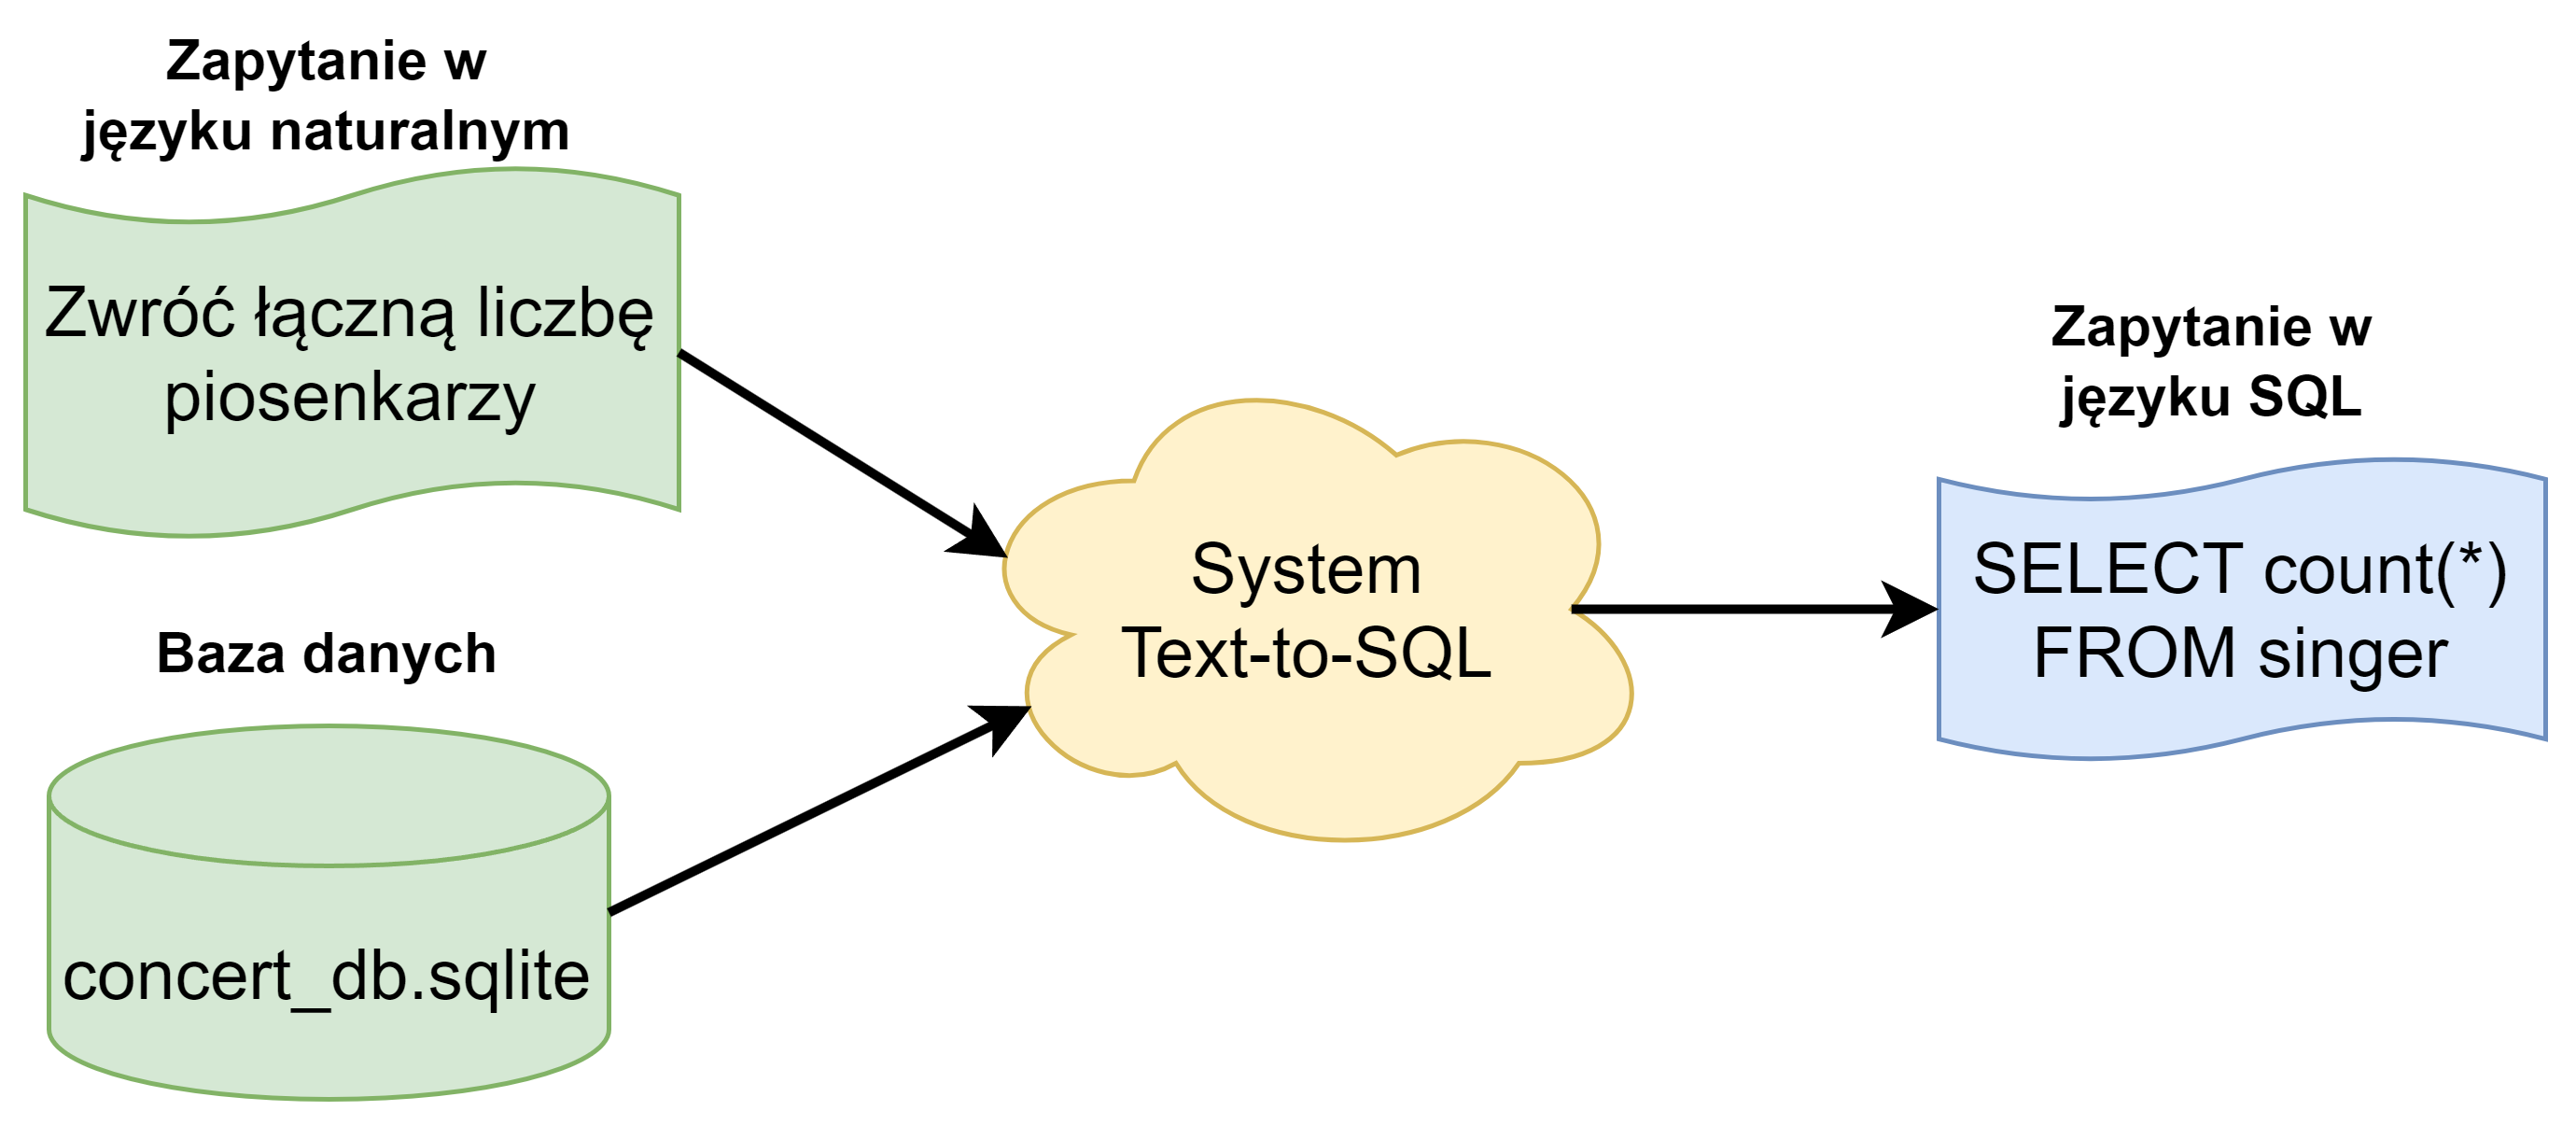
\includegraphics[width=0.8\linewidth]{images/text_to_sql.png}
  \caption{Problem \code{Text-to-SQL}}
  \label{fig:text-to-sql}
\end{figure}

Zapytanie naturalne może przyjmować wiele różnych postaci. Oczywistą formą są zdania rozkazujące, ponieważ bardzo dobrze mapują się na zapytania SQL, które mają strukturę zbliżoną właśnie do zdań rozkazujących. Równie dobrze rolę zapytań naturalnych mogą pełnić jednak zdania pytające, w których użytkownik zapytuje system o potrzebną informację. Dopuszczalne jest również wykorzystanie w tej roli bezokoliczników, czy też pojedynczych słów kluczowych.

\section{Cel i zakres pracy}
Celem niniejszej pracy dyplomowej jest wykorzystanie technik uczenia maszynowego, aby opracować rozwiązanie dokonujące tłumaczenia zapytań z języka polskiego na SQL oraz jego przetestowanie. System ten ma rozwiązywać zdefiniowany we wcześniejszej sekcji problem. W szczególności ma działać w sposób bezkontekstowy, nieumożliwiający interakcji w konwersacyjnej formie, co stanowi problem trudniejszy. Istotnym elementem testów ma być ocena użyteczności powstałego narzędzia dokonana przez potencjalnych użytkowników.

Pośrednim celem pracy, który niezbędny jest jednak by pożądane rozwiązanie stworzyć, jest opracowanie polskich zbiorów danych. Ma to zostać dokonane poprzez tłumaczenie istniejących zbiorów anglojęzycznych, w szczególności zbioru \code{Spider}, ponieważ na nim większość tego typu modeli jest uczona. W zakres pracy wchodzi przeprowadzenie eksperymentów w celu lepszego zrozumienia działania modeli \code{Text-to-SQL} oraz wybrania najbardziej obiecującego.

